\documentclass[12pt]{article}
\usepackage{fontspec}
\usepackage{polyglossia}
\usepackage{listings}
\setdefaultlanguage{russian}
\setotherlanguages{english}
\setmainfont[Mapping=tex-text]{CMU Serif}
\setmonofont[Mapping=tex-text]{Courier}

\newcommand{\englishterm}[1]{\textenglish{\texttt{#1}}}

\begin{document}
\begin{section}{Обзор фреймворков}
\begin{subsection}{ORK (OpenGL rendering kernel)}
Небольшой фреймворк для работы с OpenGL.
Реализованы следующие возможности:
\begin{itemize}
    \item автоматическая сборка мусора, основанная на умных указателях;
    \item динамическая загрузка объектов по xml-описанию;
    \item создание графа задач и его выполнение.
\end{itemize}

Также содержит примитивы линейной алгебры и примитивы для работы с OpenGL.
\end{subsection}

\begin{subsection}{Proland}
Фреймворк для эффективного и корректного отображения местности на глобусе, включая рельеф, дороги и водоемы. В своей реализации активно опирается на ORK.

Состоит из ядра и набора плагинов. Каждый плагин содержит объекты для работы с некоторой предметной областью:
\begin{itemize}
    \item terrain для рельефа;
    \item atmo для атмосферы;
    \item graph для графов (и дорог в частности)
    \item и т.д.
\end{itemize}
Большинство плагинов не зависят друг от друга.

Для решения поставленной задачи (определение высоты точки по ее угловым координатам) необходимо использовать плагин terrain и его зависимости.
\end{subsection}
\end{section}

\begin{section}{Процесс сборки}
Для корректной работы Proland необходимо подключить правильно сконфигурированную библиотеку LIBTIFF. При сборке LIBTIFF из исходных файлов требуется в конфигурационном файле nmake.opt раскомментировать следующие строки, указав корректный путь к библиотеке zlib:
\begin{lstlisting}
ZIP_SUPPORT	 = 1
ZLIBDIR 	 = <some path>
ZLIB_INCLUDE = -I$(ZLIBDIR)
ZLIB_LIB 	 = $(ZLIBDIR)/zlib.lib
\end{lstlisting}

Фреймворк ORK имеет собственную реализацию \englishterm{shared\_ptr}. Для того, чтобы использовать стандартный указатель, следует выставить директиву препроцессора USE\_SHARED\_PTR.
Также этот фреймворк включает в себя небольшую библиотеку для чтения xml -- TinyXML. Она может использовать свою реализацию строк. Для того, чтобы использовать стандартные строки, следует выставить директиву препроцессора TIXML\_USE\_STL.

Итоговые директивы препроцессора:
\begin{itemize}
    \item USE\_SHARED\_PTR;
    \item \_CRT\_SECURE\_NO\_WARNINGS (только для proland);
    \item PROLAND\_API=\_\_declspec(dllexport/dllimport);
    \item ORK\_API=\_\_declspec(dllexport/dllimport);
    \item TIXML\_USE\_STL.
\end{itemize}
\end{section}

\begin{section}{Основные понятия}
Terrain плагин позволяет работать с растровыми и векторными данными на плоскости и на сфере. Для работы со сферой применяется методика \textit{cube mapping}. Высотные данные должны находиться в файле DEM.dat для модели на плоскости или DEM[1-6].dat для сферической модели. Каждый файл соответствует некоторой грани куба (для сферического случая).

\begin{figure}[h]
    \centering
    \begin{minipage}{0.45\textwidth}
        \centering
        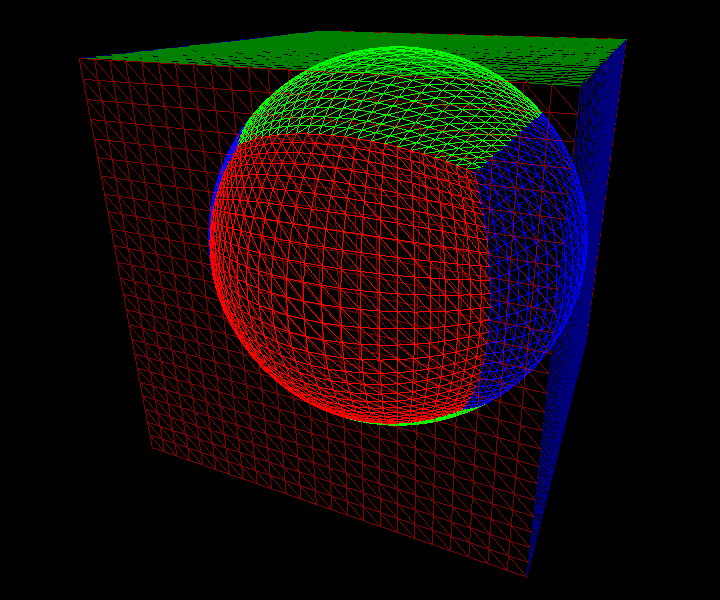
\includegraphics[width=\linewidth]{cube_mapping}
        \caption{Соответствие граней куба областям сферы}
        \label{fig:mapping}
    \end{minipage}\hfill
    \begin{minipage}{0.45\textwidth}
    \centering
        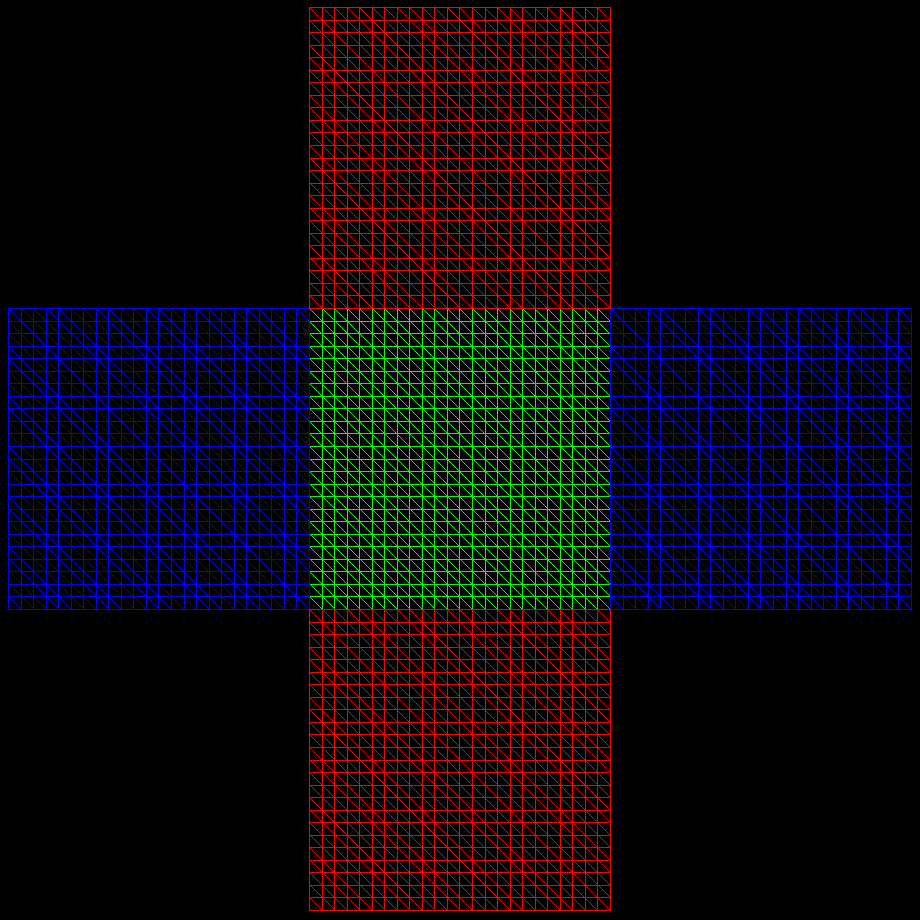
\includegraphics[width=\linewidth]{cube_net}
        \caption{Развертка куба}
        \label{fig:net}
    \end{minipage}
\end{figure}

Данные для некоторой квадратной области (далее: \textit{исследуемая область}) хранятся с помощью \textit{квадродерева}. Каждый уровень состоит из одного или более \textit{quad}. \textit{Тайлом} называется информация, соответсвующая некоторому quad.
Первый уровень квадродерева содержит ровно один quad. При переходе на следующий уровень quad либо разбивается на 4 дочерних, либо не разбивается вообще.

\begin{subsection}{Системы координат}
При работе с quad и тайлами используются две системы координат: логическая и физическая. В каждой из них quad задается тройкой $(l, x, y)$, где $l$ -- номер уровня в квадродереве, $x, y$ -- координаты левого нижнего угла quad в текущей системе координат.

\begin{paragraph}{Логическая система координат}
Началом координат является левый нижний угол. Правый верхний угол имеет координаты $(2^l, 2^l)$, где $l$ -- порядковый номер уровня в квадродереве. Каждый quad имеет размеры 1x1, таким образом, число quad на уровне -- $4^l$.
\end{paragraph}

\begin{paragraph}{Физическая система координат}
Началом координат является центр квадрата. Левый нижний угол имеет координаты $(-\frac{l}{2}, -\frac{l}{2})$, правый верхний соответственно $(\frac{l}{2}, \frac{l}{2})$, где $l$ -- длина стороны исследуемой области.
\end{paragraph}

\begin{paragraph}{Географическая система координат}
Полярная система координат, используемая для позиционирования на земле.
Широта лежит в диапазоне от $-90$ градусов (или $90$ градусов южной широты) до $90$ градусов (или $90$ градусов северной широты).
Долгота лежит в диапазоне от $-180$ градусов (или $180$ градусов западной долготы) до $180$ градусов (или $180$ градусов восточной долготы).
\end{paragraph}
\end{subsection}

\begin{subsection}{Хранилище тайлов (\englishterm{TileStorage}) и кеши (\englishterm{TileCache)}}
С каждым quad можно ассоциировать некоторую растровую или векторную информацию. Растровая информация может храниться в двух формах: в виде 2D-текстур для дальнейшего эффективного отображения (\englishterm{GPUTileStorage}) или в виде массивов чисел (\englishterm{CPUTileStorage}).
Хранилище имеет заранее заданный размер. Тайлы могут иметь непустую границу (в представленных DEM-файлах она составляет 2 пикселя). Это порождает некоторую избыточность, но бывает полезно в некоторых случаях (например, чтобы избежать артефактов при фильтрации текстур или генерации соседних тайлов).

С каждым хранилищем можно ассоциировать кеш, который будет следить за тем, какие из тайлов используются. Если тайл не используется, он может быть удален кешом из хранилища в произвольный момент времени.
Тайл можно получить методом \englishterm{TileCache::getTile}, после чего число владельцев тайла увеличивается на один. После вызова метода \englishterm{TileCache::putTile} число владельцев уменьшается на один.
Тайл может быть корректно удален (например, при завершении программы и очистке памяти), только если у него нет ни одного владельца.
\end{subsection}
 
\begin{subsection}{Производители тайлов (\englishterm{TileProducer)}}
Для хранения высотных данных используется дельта-кодирование. Таким образом, тайл высотных данных (\textit{высотный тайл}, \textit{elevation tile}) уровня $l$ может быть построен из высотного тайла уровня $l - 1$ и соответствующего \textit{добавочного тайла} (\textit{residual tile}) уровня $l$.
Для этого родительский высотный тайл разбивается на 4 дочерних и к ним добавляются добавочные тайлы.

Для построения высотных тайлов существует два класса: \englishterm{ElevationProducer} и \englishterm{CPUElevationProducer}. Первый используется для создания 2D-текстур и хранит тайлы в \englishterm{GPUTileStorage}. Второй используется для хранения высот в виде отдельных значений и хранит тайлы в \englishterm{CPUTileStorage}.
DEM-файлы содержат в себе заранее подготовленные добавочные тайлы, которые могут быть считаны при помощи класса \englishterm{ResidualProducer}.

Один и тот же кеш может быть использован несколькими производителями. Для этого каждому производителю дается уникальный номер, а тайл внутри кеша характеризуется четверкой чисел $(p, l, x, y)$, где $p$ -- номер производителя, $l$ -- номер уровня в квадродереве, $x, y$ -- координаты левого нижнего угла тайла в текущей системе координат.
\end{subsection}

\begin{subsection}{Задачи (\englishterm{Task}) и графы задач (\englishterm{TaskGraph})}
Так как выполение некоторых действий может занимать достаточно продолжительное время (например, чтение добавочных тайлов из файла с диска), активно применяются многопоточность и отложенные вычисления. Для этого создаются задачи, которые будут выполнены планировщиком в некоторый момент времени.
Класс \englishterm{MultithreadScheduler} представляет собой реализацию планировщика для нескольких потоков.

Некоторые действия должны происходить в некотором порядке (например, для построения высотного тайла, нужно построить высотный тайл предыдущего уровня, а также один или несколько добавочных тайлов). Для решения этой проблемы используются графы задач.
Между задачами можно создавать зависимости, таким образом давая планировщику возможность понять, можно ли выполнить данную задачу или нет.

Например, для построения высотного тайла уровня $l$, нужно построить родительский тайл (если он еще не построен), а также один или несколько добавочных тайлов. Создается граф задач, в который добавляются задачи построить высотный тайл, задачи построить добавочные тайлы, добавляются соответсвующие зависимости.
В тот момент, как запрашивается родительский высотный тайл, в граф будет добавлена задача его создания и зависимость от результата его исполнения. Если для построения родительского тайла требуется построить еще какие-то тайлы, задачи на их построение также будут добавлены в граф.

Одно и то же задание можно добавлять в несколько графов задач. Это может потребоваться, например, если некоторый тайл уже кем-то запрошен, но также требуется для выполнения некоторого действия.
\end{subsection}

\begin{subsection}{DEM-файлы}
DEM-файл хранит в себе заранее подготовленные добавочные тайлы и дополнительную служебную информацию.
В начале файла идет заголовок, в нем записаны следующие значения:
\begin{enumerate}
    \item минимальный уровень в квадродереве;
    \item максимальный уровень в квадродереве;
    \item размер тайлов в пикселях минус 5 \footnote{Proland внутри себя активно использует тот факт, что граница тайла имеет ширину в два пикселя. Таким образом, минимально возможный тайл имеет размер 5x5.};
    \item начальный уровень в квадродереве;
    \item и другое.
\end{enumerate}

После заголовка идет массив сдвигов, по которым располагаются добавочные тайлы. Каждый тайл записан в формате TIFF. На каждый пиксель отводится по 16 бит.
Сдвиг для конкретного тайла может быть вычислен, как функция от идентификатора тайла $(l, x, y)$, а также значений, указанных в заголовке.

Некоторая область может описывать не одним DEM-файлом. Например, если есть уточняющие данные для некоторого региона, то соответсутвующее им квадродерево может быть включено в исходное.

\begin{paragraph}{Создание собственных DEM-файлов}
Для самостоятельного создания DEM-файлов используются методы \englishterm{preprocessDem} для случая плоскости и \englishterm{preprocessSphericalDem} для случая сферы. В первом случае генерируется ровно один DEM.dat файл, во втором генерируются DEM[1-6].dat файлы.
На вход этому методу передается некоторая реализация интерфейса \englishterm{InputMap}. Метод \englishterm{InputMap::getValue} выдает значение пикселя по его координатам.

Таким образом, существует возможность подгатавливать DEM-файлы из своих данных. Например, это может быть даже текстовый файл, в котором записаны координаты точек и их высоты.
\end{paragraph}
\end{subsection}
\end{section}

\begin{section}{Методика решения}
\begin{subsection}{Высотные запросы}
Метод \englishterm{CPUElevationProducer::getHeight} позволяет отвечать на высотные запросы с некоторой точностью. Координаты точки задаются в физической системе координат.

Процесс перевода координат в полярной системе координат (широта-долгота) в локальную физическую систему координат выглядит следующим образом:
\begin{enumerate}
    \item перевести координаты точки из полярной системы в декартову;
    \item определить, на какой грани куба находится образ точки;
    \item перевести декартовы координаты точки в систему координат грани куба (домножить на матрицу поворота);
    \item построить образ точки на грани куба (методом \englishterm{SphericalDeformation::deformedToLocal}).
\end{enumerate}

\begin{subsection}{Курсор}
Класс \englishterm{elevation\_cursor} представляет из себя курсор, обладающий следующим интерфейсом:
\begin{itemize}
    \item \englishterm{void set\_position(const lat\_lon\_d\&)} -- установить позицию курсора в географической системе координат;
    \item \englishterm{double get\_current\_height() const} -- узнать высоту с текущим уровнем детализации;
    \item \englishterm{size\_t get\_current\_level() const} -- узнать текущий уровень детализации;
    \item \englishterm{void leave\_request(size\_t)} -- оставить запрос на повышение уровня детализации.
\end{itemize}

Последний метод принимает на вход целочисленные значения в диапазоне от минимального уровня квадродерева до максимального.
\end{subsection}
\end{section}
\end{document}